\clearpage
\begin{column}{ミニ研究~東京都心部の道路網におけるsecond-best pricing~}

東京都心部（山手線の内側）の道路ネットワークを対象に，以下の分析を行った．

(1) Day-to-day ダイナミクスシミュレーションに基づき，
収束後の UE 状態における総旅行時間，リンクごとの旅行時間および交通量を算定した．

(2) 総旅行時間の短縮（SO 配分の目的関数）に基づいて
Pigouvian 課金を導出し，その課金を導入した状態で
Day-to-day ダイナミクスシミュレーションを行った場合，
総旅行時間が SO 配分と一致することを確認した．

(3) 課金可能リンクに限定して Pigouvian 課金を導入した場合について，
総旅行時間や社会的余剰の変化を分析した．

なお，使用したデータは山手線内側周辺の交通ネットワークデータ（幹線道路）と
2019年PT調査を基にしたOD交通量データである．
PT調査は標本調査であるため，
PTによって得られたOD需要は300倍している．
どの地域からの出発が多いか図示してみたところ，
文京区のあたりが最も多くなっていた．

\begin{center}
  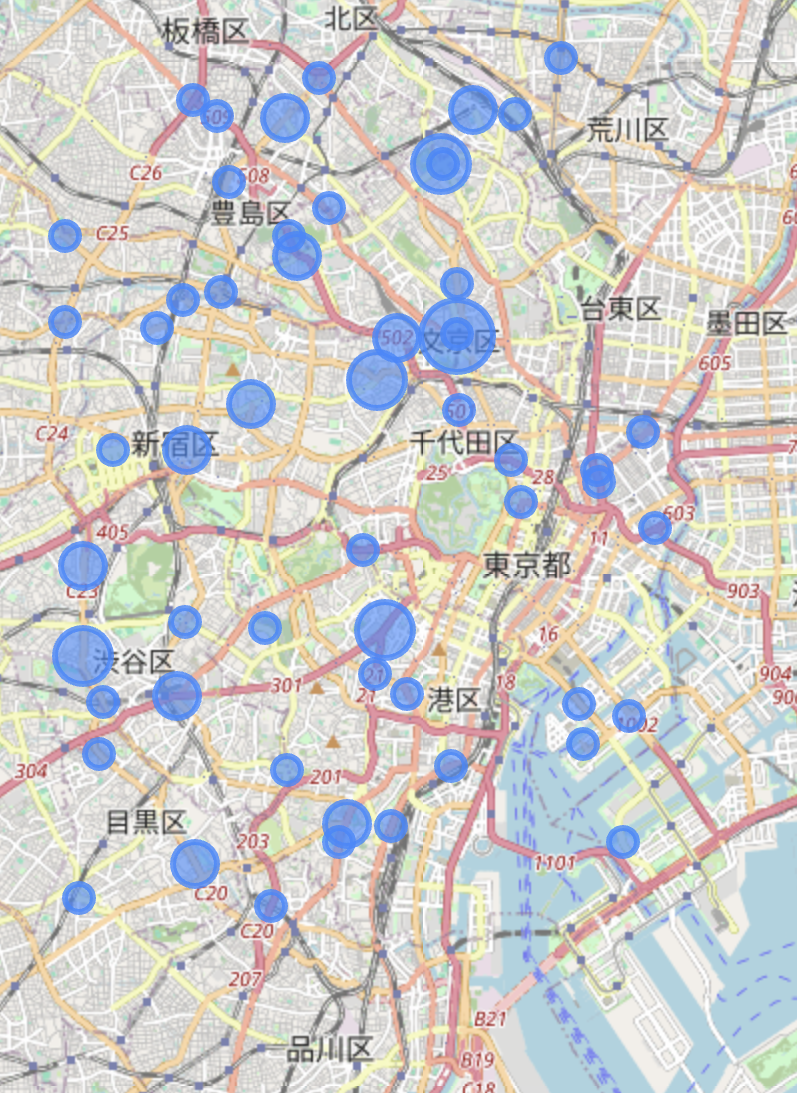
\includegraphics[width=0.5\linewidth]{assets/assignment/fig_column2/origin_distribution.png}
  \captionof{figure}{発地分布}
\end{center}

\vspace{4mm}

\textbf{(1) Day-to-day ダイナミクスによるUE状態の算定}

今回，day-to-dayダイナミクスは

\[
x^{t+1} = (1-\eta)x^t + \eta \cdot \mathrm{AON}(c(x^t)+\tau)
\]

という更新則に基づく．
これは，前日の経路コストを踏まえてAON配分が行われるが，
実際にその経路に動くのは一部
（今回であれば，10\%）であるということを示す．

AON配分は離散的な配分であり，
AON配分されるリンクが変化するたびに
総旅行時間は均衡点の付近でジグザグと変化する．

実際にこの更新則のもとで計算を回すと，
23100の総トリップは図のように収束し，
総旅行時間は2150.1078 [h$\cdot$台] となる．

\begin{center}
  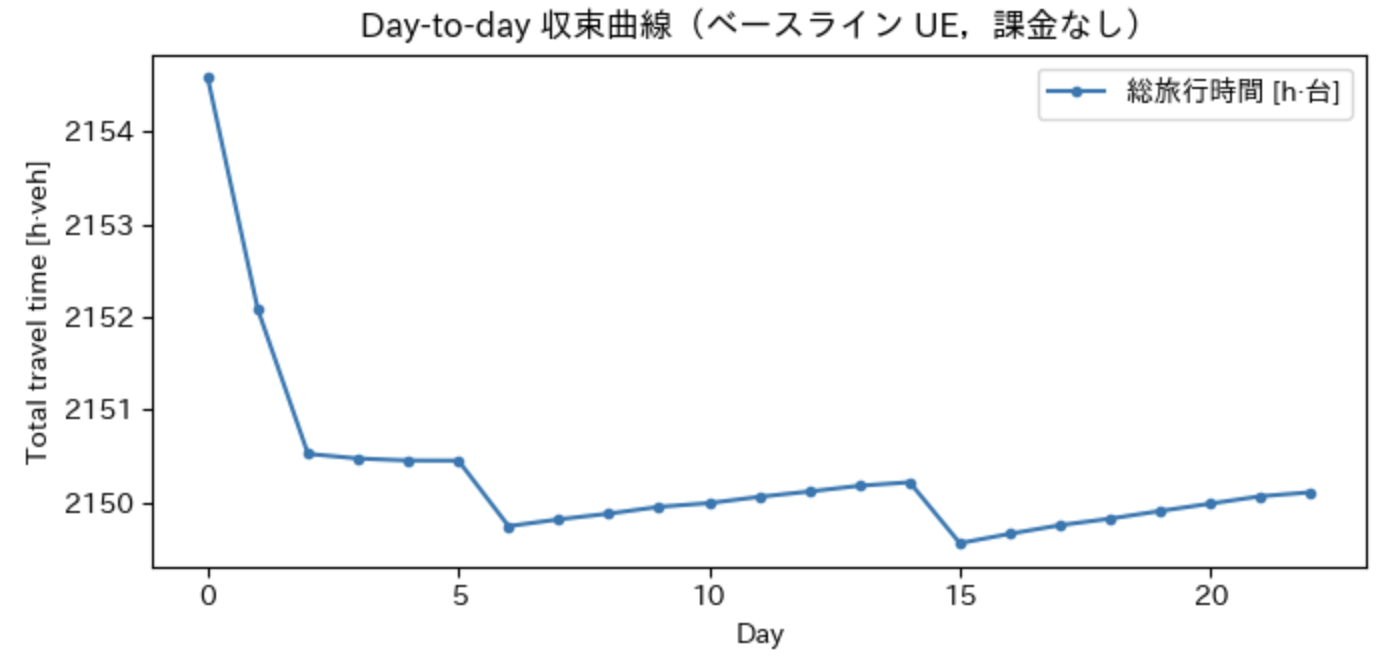
\includegraphics[width=\linewidth]{assets/assignment/fig_column2/day_to_day_ue.png}
  \captionof{figure}{Day-to-dayダイナミクスの収束}
\end{center}


また，均衡に達した際の道路の混み具合
（赤が混んでいる）を示すマップは以下のようになった．

\begin{center}
  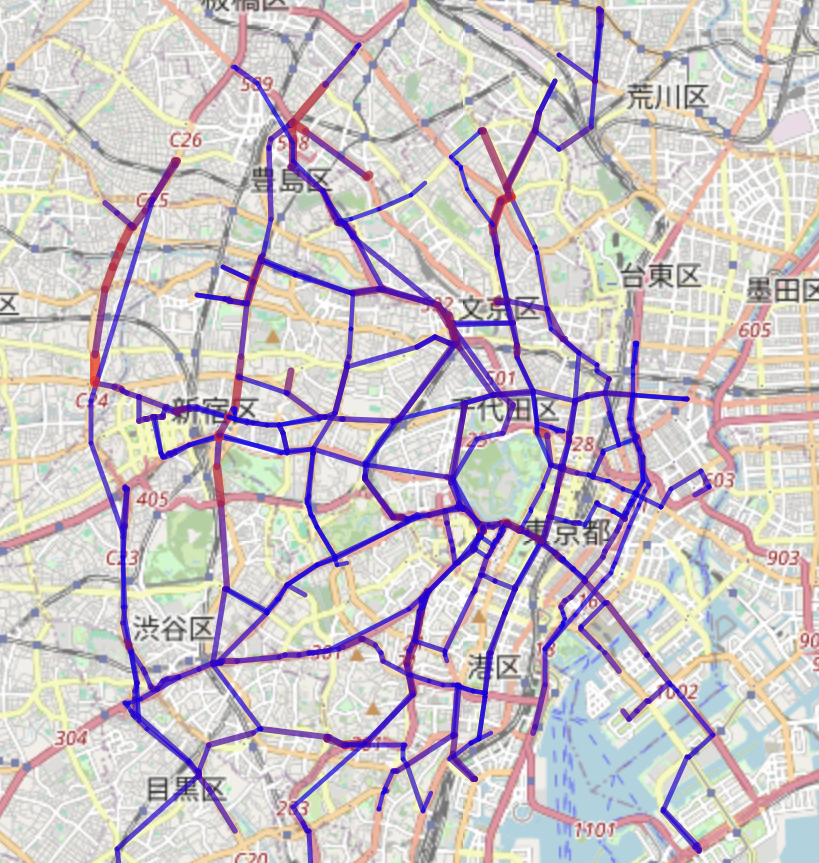
\includegraphics[width=0.5\linewidth]{assets/assignment/fig_column2/congestion_map.png}
  \captionof{figure}{UE状態におけるリンク混雑度}
\end{center}

さらに，最も混雑していた文京区向丘周辺を拡大すると，
以下のようになった．

\begin{center}
  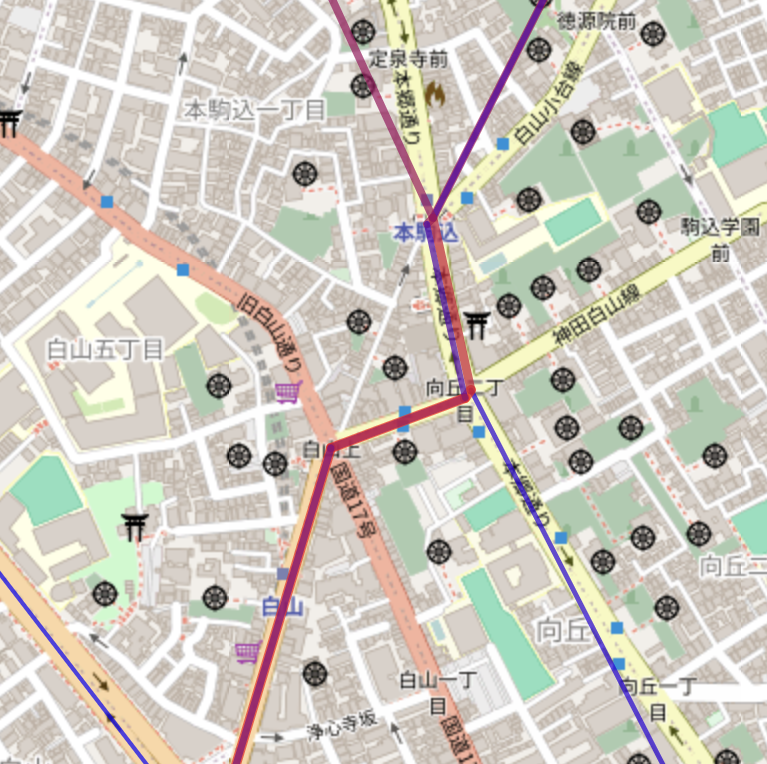
\includegraphics[width=0.5\linewidth]{assets/assignment/fig_column2/mukogaoka_map.png}
  \captionof{figure}{文京区向丘周辺の混雑状況}
\end{center}


混雑しているリンクはどちらかといえば北側に集中しており，
この過程のもとで最も混雑しているリンクは
文京区向丘周辺となった．

東京都心部の道路ネットワークは
千代田区を中心に放射状に広がっており，
それらをつなぐ環状線など，
複数の道路が入り込む場所の道路容量が少ない場合，
混雑する傾向にあり，
それが需要が多い北側であるとより顕著になる．

\vspace{4mm}

\textbf{(2) SO配分と課金状態でのDay-to-dayダイナミクス}

先ほどとは異なり，
総旅行時間の最小化を目的関数にとると，

\[
t_a(x_a) + t'_a(x_a)\cdot x_a
\]

をリンクコストとしてFrank-Wolfe法を用い
均衡を求めることができる．

総旅行時間は

\[
T_{\mathrm{SO}} = 2146.8598 \ [\mathrm{h}\cdot\mathrm{台}]
\]

となり，
その均衡を達成するために必要な課金額の最大値は
時間で表すと0.17分となる．

リンクごとに適切な課金を施し，
day-to-dayダイナミクスを回していくことで
SOと同じ配分結果を得ることができる．
これはほかでもなく，
課金によって外部性が内部化されている事を表す．

\begin{center}
  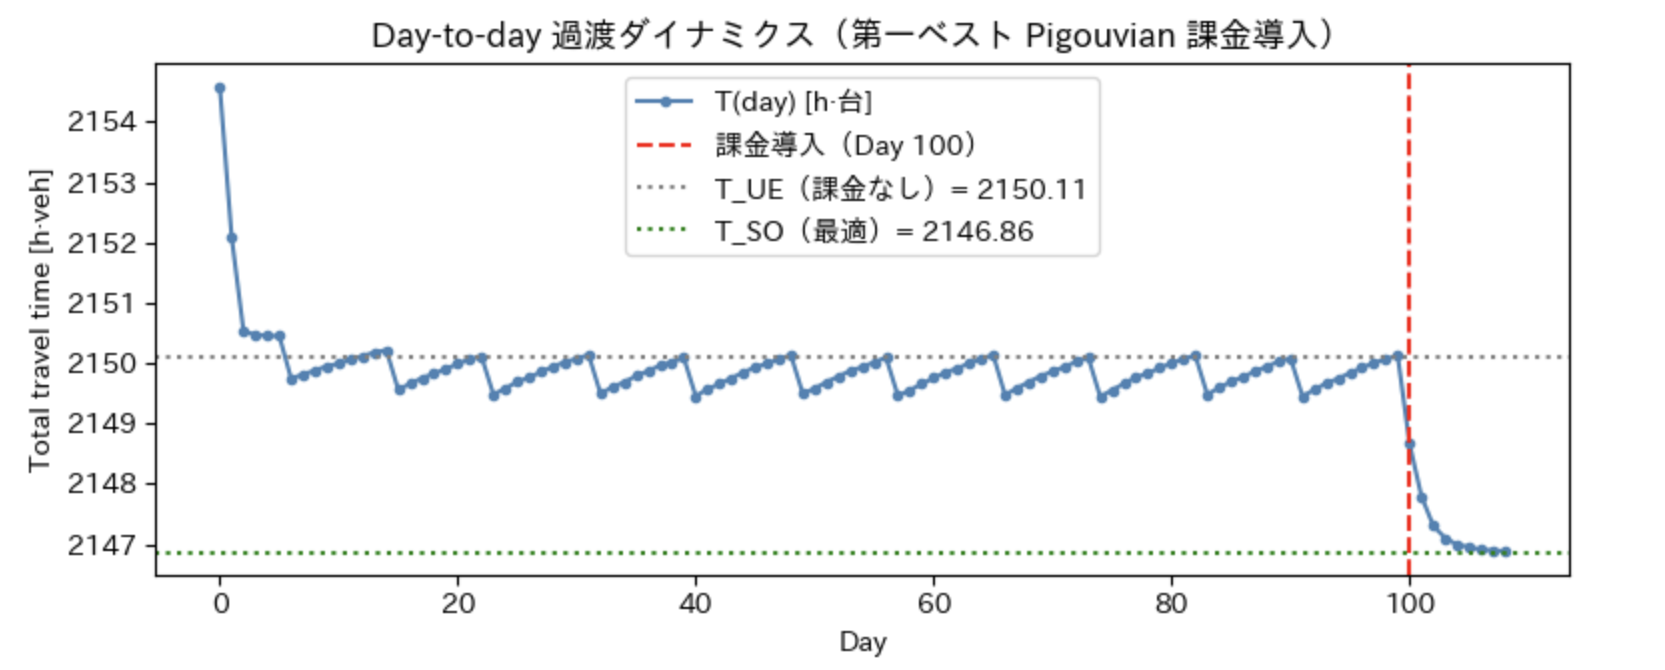
\includegraphics[width=\linewidth]{assets/assignment/fig_column2/day_to_day_first_best.png}
  \captionof{figure}{First-best課金下でのDay-to-dayダイナミクス}
\end{center}


この仮定のもとで最も課金されたリンクは
文京区本駒込ー動坂間のリンクであった．

文京区からの発地が多かったことや
この辺りのリンクのcapacityが小さいことなどから，
混雑し，かつ重要であるリンクに
より多くの課金がされることが確認できる．

\begin{center}
  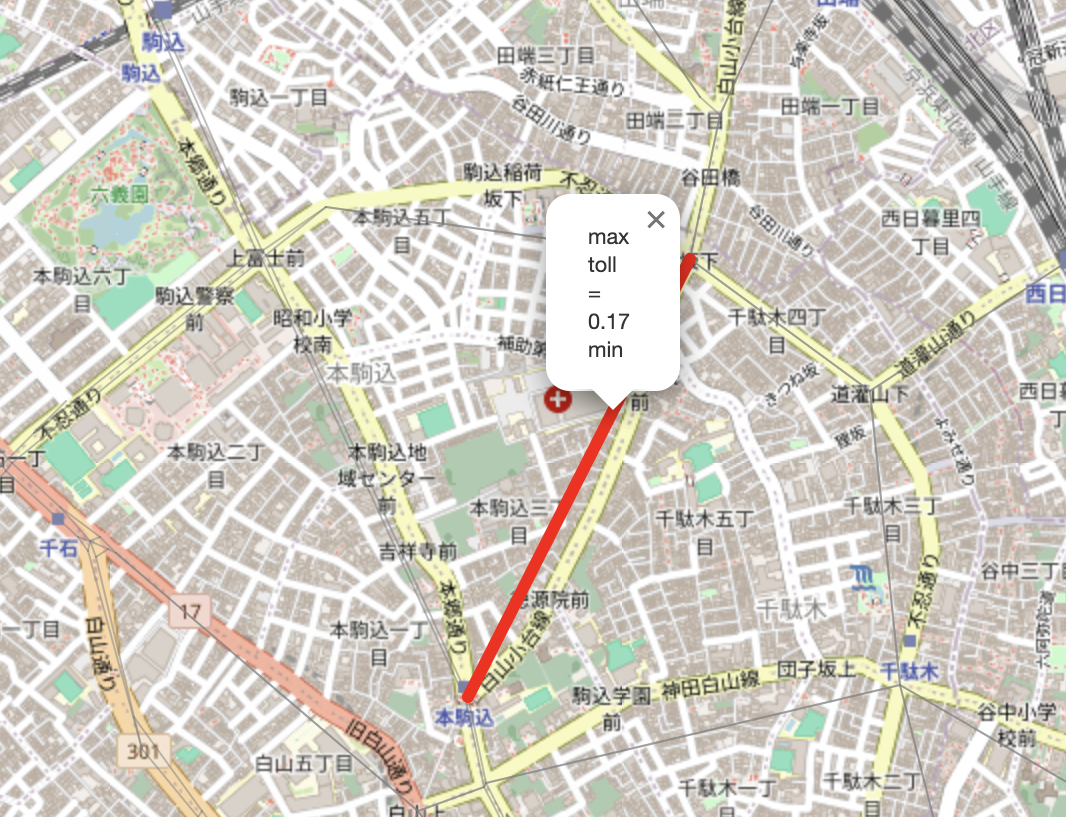
\includegraphics[width=0.5\linewidth]{assets/assignment/fig_column2/max_toll_link.png}
  \captionof{figure}{最大課金リンク周辺}
\end{center}


\vspace{4mm}

\textbf{(3) 課金可能リンクへの限定}

今回，
課金可能なエッジ数は全体のリンクの28\%であった
（国道などの幹線道路及び高速道路）．

それらのリンクに先ほど求めた
First-bestな課金を施すと，
総旅行時間は2150.0788 [h$\cdot$台] となり，
UEの時とほぼ変わらなくなってしまった．

先ほどのように
狭くて需要が集中しているリンクに
直接の課金ができないためであると考えられる．

\end{column}

\clearpage
